\chapter{Circuit Design}
\label{chap:10}

\section{Linear Method}
\subsection{Block Diagram}
This is the block diagram. Instead of Cuff, an NIBP Simulator is applied and the MCU read the sensor data through I2C and control the Air Pump through the Pump Switch Circuit and the restriction of the Valve via Valve Control Circuit. 

\begin{figure}[h]
    \centering 
    \captionsetup{justification=centering}
    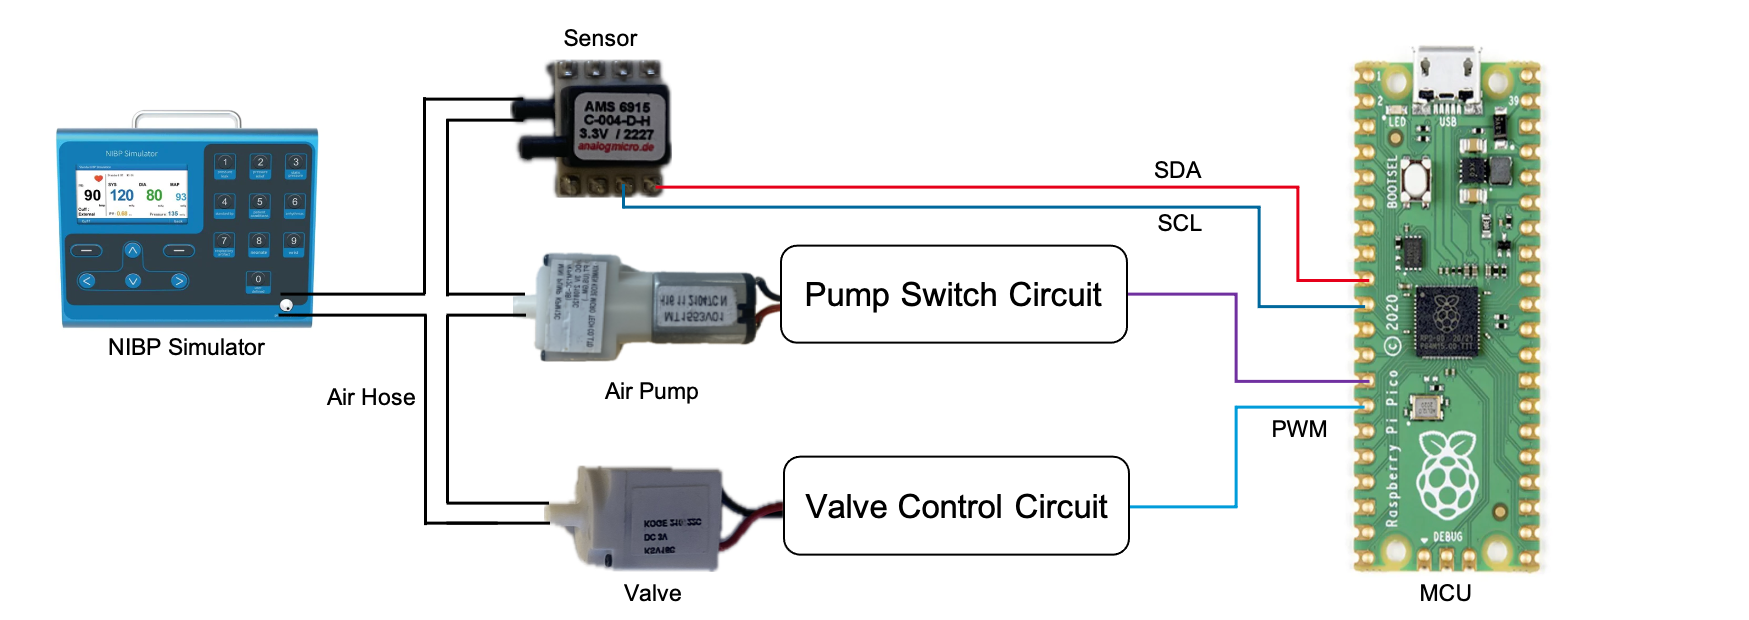
\includegraphics[width=\textwidth]{img/blockdiagram_lin.png}
    \caption{a nice plot}
    \label{fig:mesh1}
\end{figure}

% 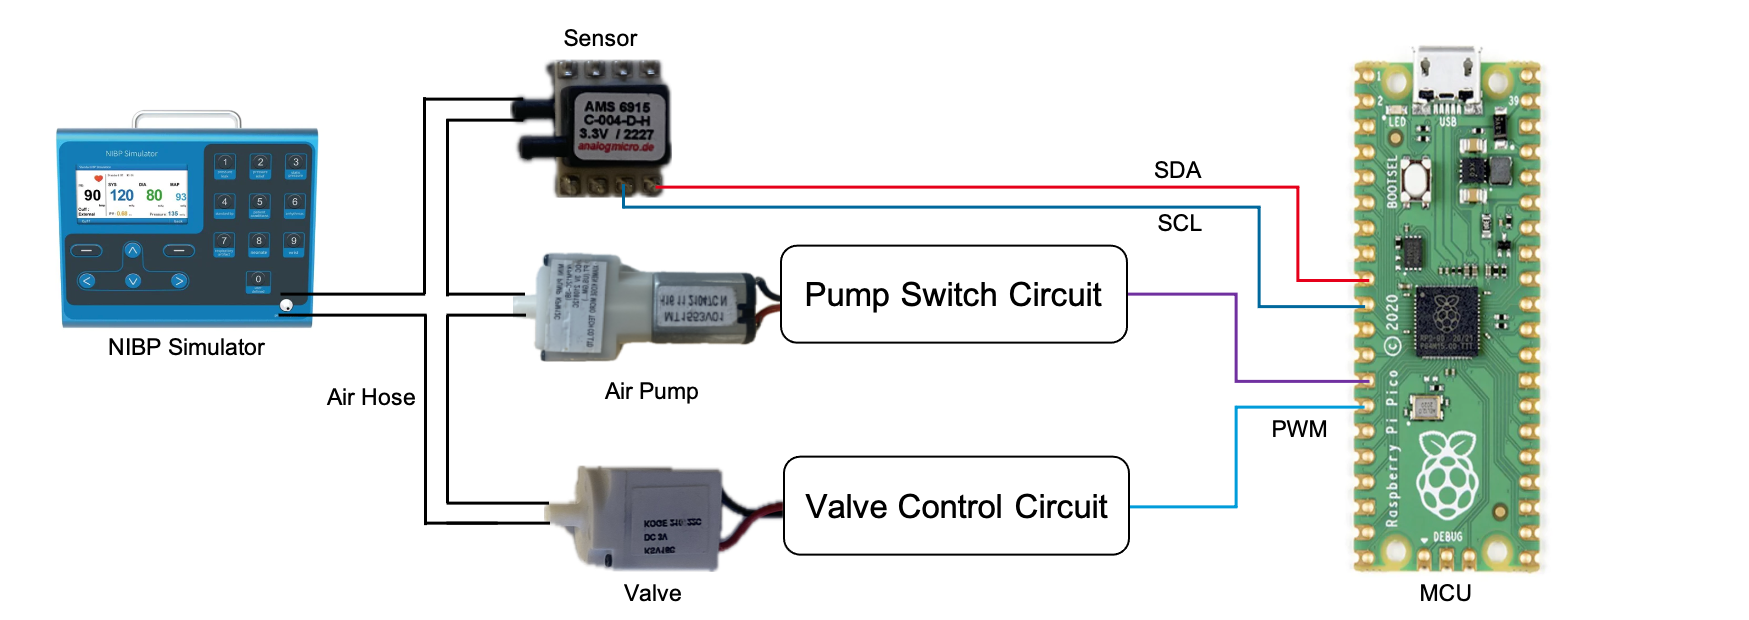
\includegraphics[width=\textwidth]{img/blockdiagram_lin.png}
\subsection{Schematic}
As it shown in Figure 4.2, the circuit contains 5 parts, namely MCU, Power supply circuit, valve control circuit, pump switch circuit and a sensor. 

Here are detail of the main components. As the start point, I set the simulator to a standard blood pressure which is shown in the blue table, the systolic pressure is and .... As for sensor, I applied ams6915 it can measure the air pressure from 0 to 300 mmHg and has a sample rate of 200Hz

\begin{figure}[h]
    \centering
    \captionsetup{justification=centering}
    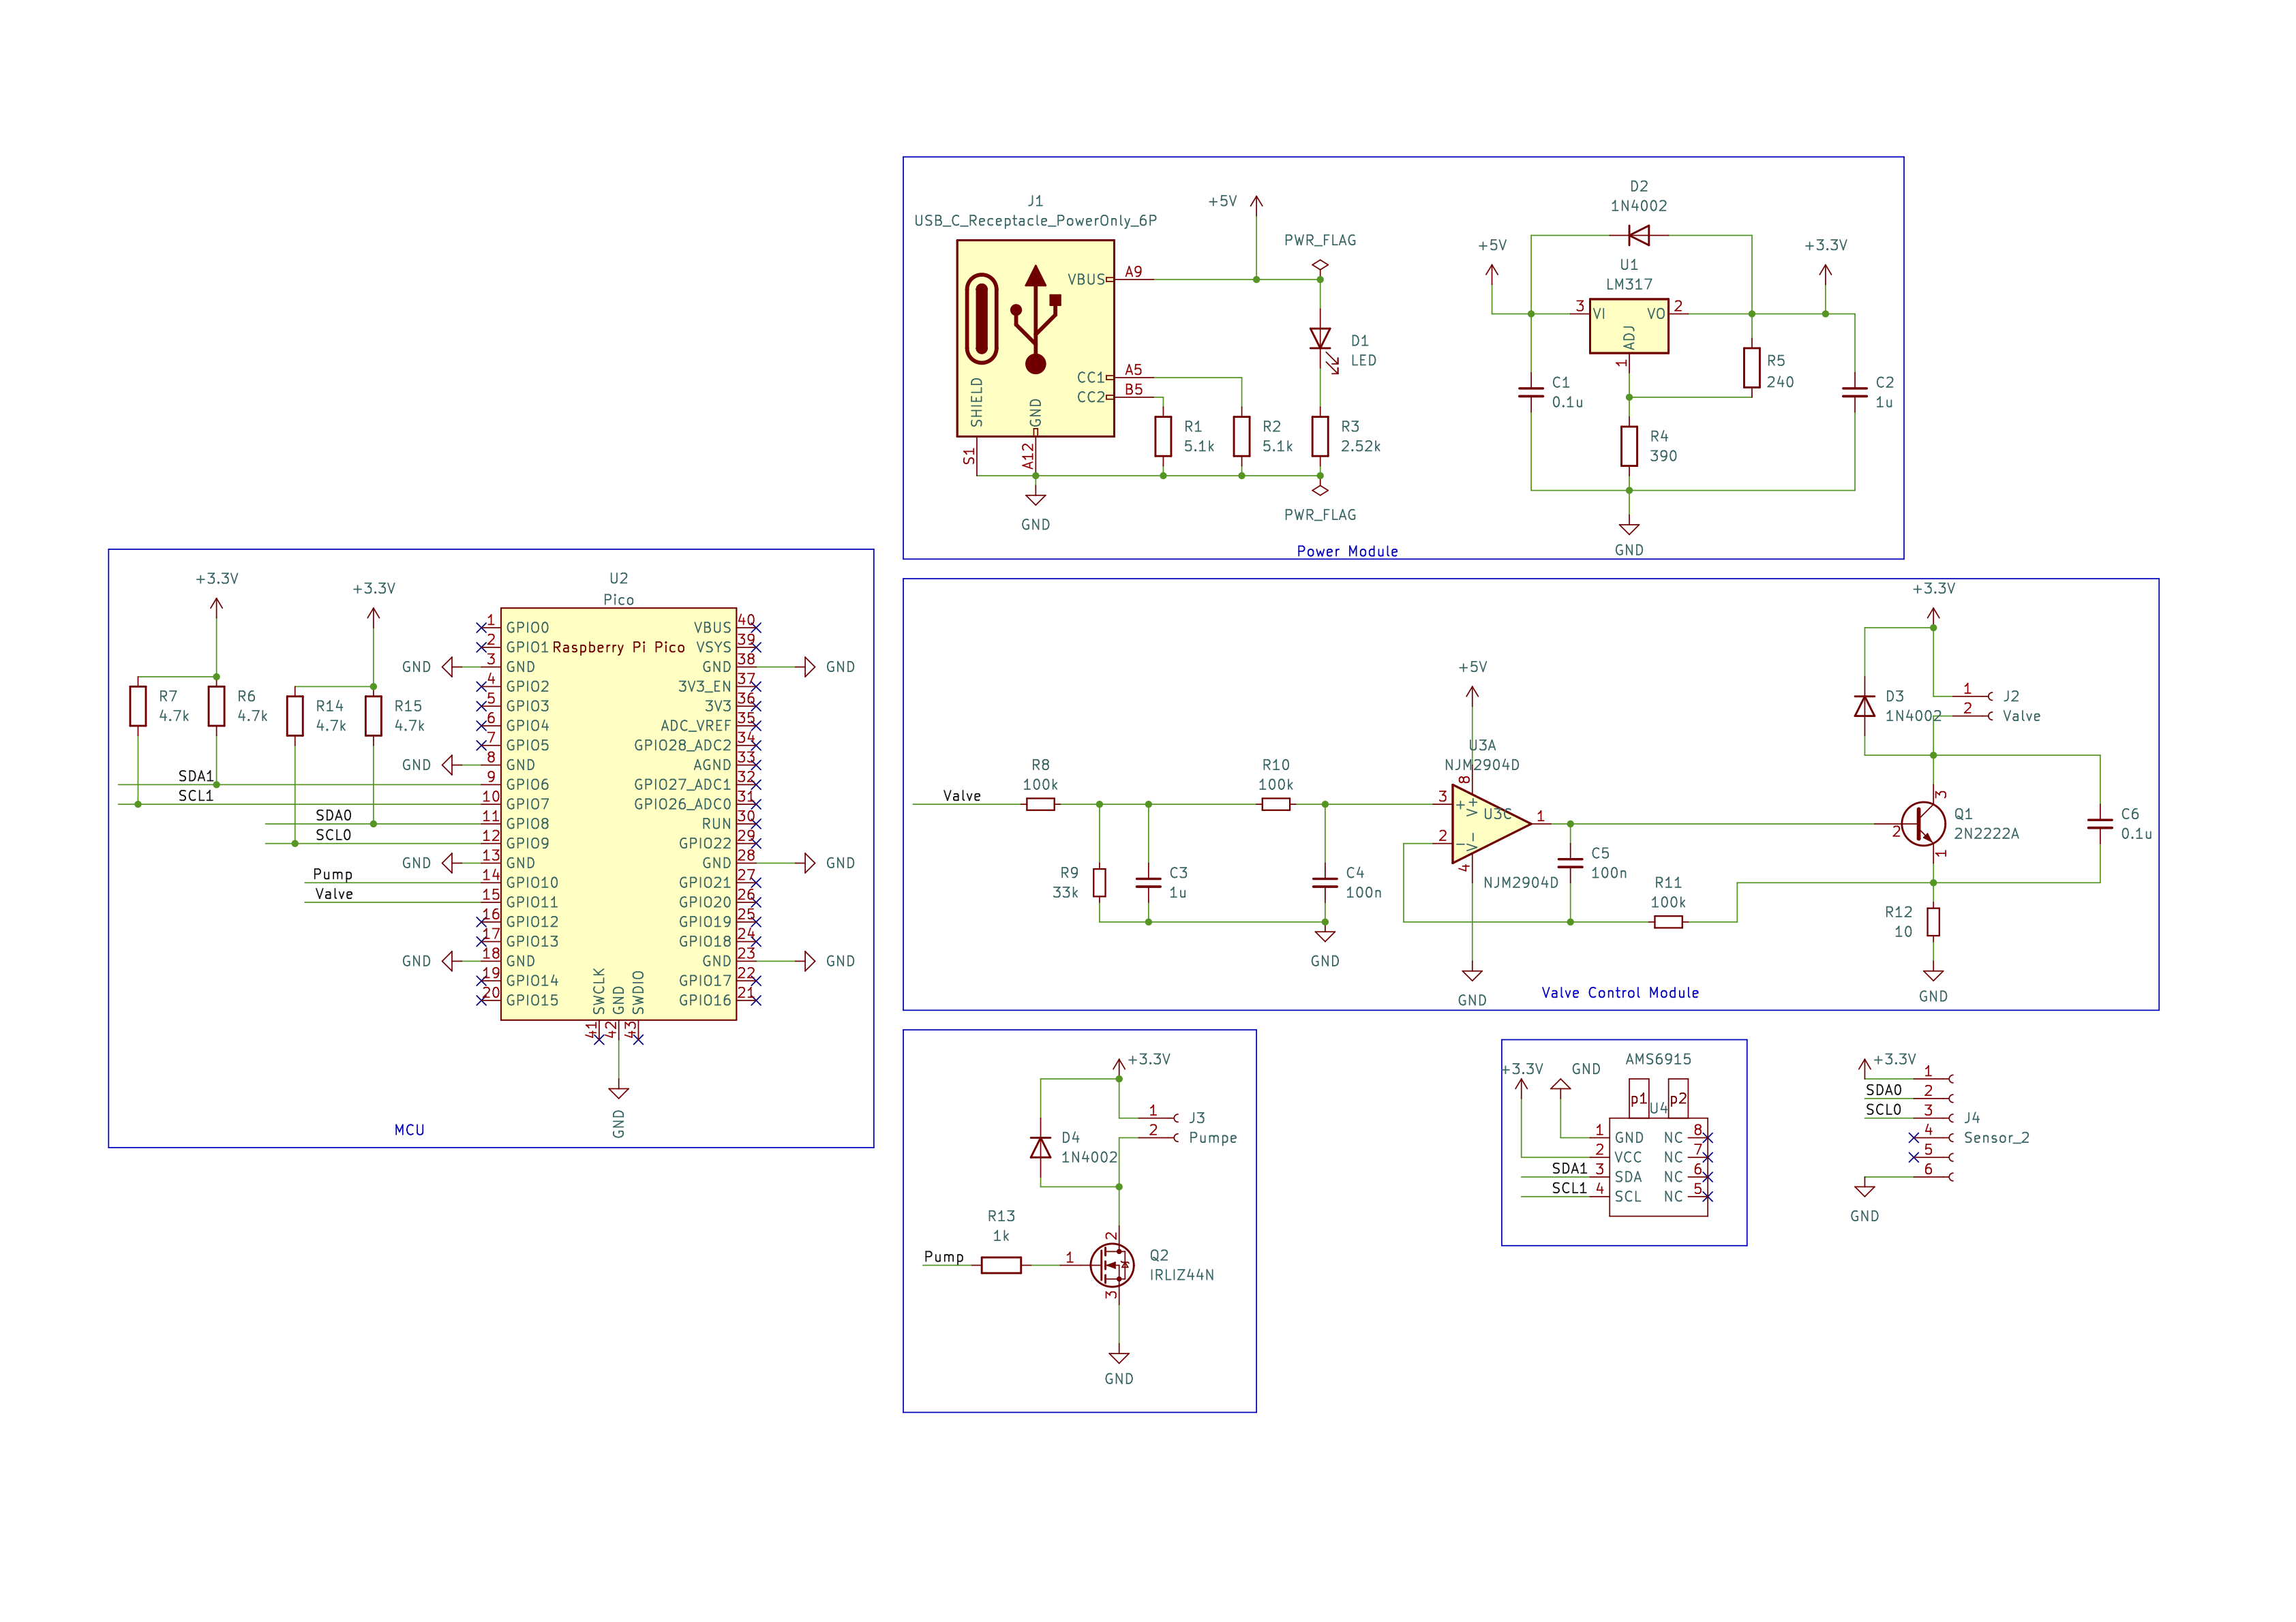
\includegraphics[width=0.75\textwidth]{img/schematic.png}
    \caption{a nice plot}
    \label{fig:mesh1}
\end{figure}

\subsection{MCU}
To have the best performance of the whole system, the Raspberry Pi Pico is applied as the micoroprocessor. It is an RP2040-based microcontroller board. The ARM Cortex-M0+ processor is a very low gate count, highly energy efficient processor that is intended for microcontroller and deeply embedded applications that require an area optimized, low-power processor.

\subsection{Pump Switch Circuit}
The MCU controls the on and off of the air pump through the pump switch circuit. A mosfet has many advantages compare to relay. In our case, a mosfet is applied.


\subsection{Valve Control Circuit}
\subsubsection{Proportional Valve}
To have a controllable restriction of the valve, a proportional valve is applied. The restriction of the proportional valve could be controlled by the current flows. In our case, the restriction is controlled by the PWM signal.

\subsubsection{PWM}
It stands for Pulse-Width-Modulation, with this techonology, the MCU could generate different levels of voltage by changing the duty circle. 

The generated PWM signal would be divided first and filtered by a second order filter. Through the operational amplifier the BJT would be conducted and the current flows through the BJT would be controlled by the filtered PWM signal.



\subsection{Power Supply Circuit}
The generated PWM signal would be divided first and filtered by a second order filter. Through the operational amplifier the BJT would be conducted and the current flows through the BJT would be controlled by the filtered PWM signal.

\section{Differential Method}
\subsection{Block Diagram}
This is the Block Diagram of Differential Method systems. It combines two linear systems together.
This is the Block Diagram of Differential Method systems. It combines two linear systems together.
\begin{figure}[h]
    \centering 
    \captionsetup{justification=centering}
    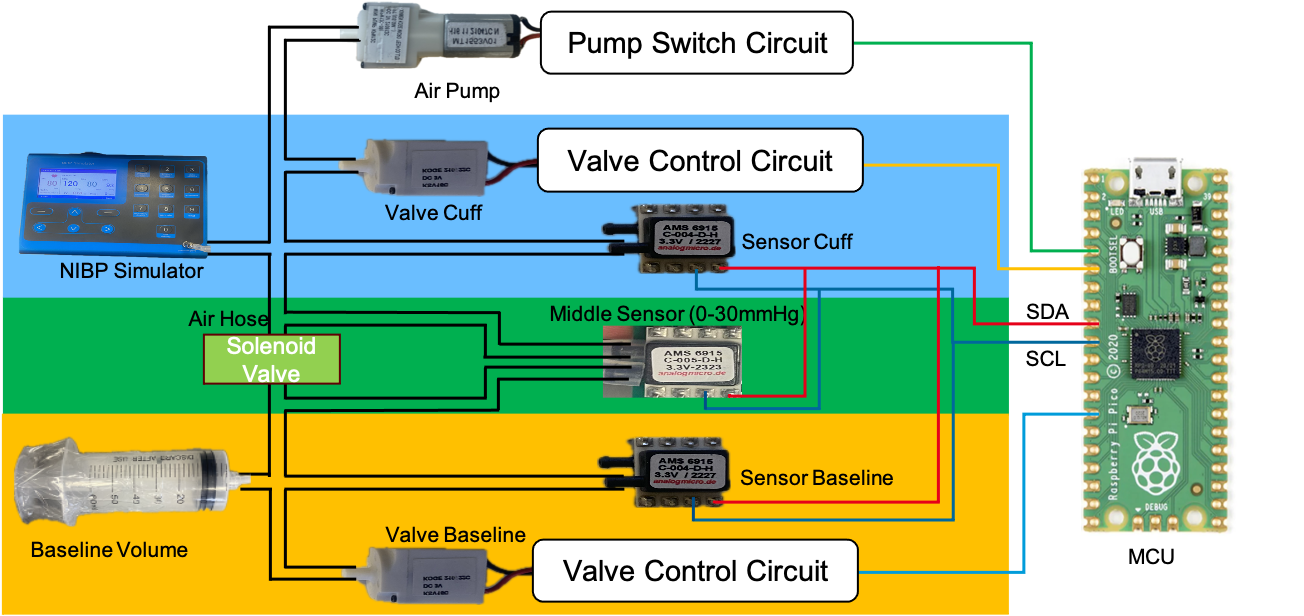
\includegraphics[width=0.75\textwidth]{img/blockdiagram_diff.png}
    \caption{a nice plot}
    \label{fig:mesh1}
\end{figure}

\subsection{Schematic}

Here is the schematic of Differential systems 
\begin{figure}[h]
    \centering
    \captionsetup{justification=centering}
    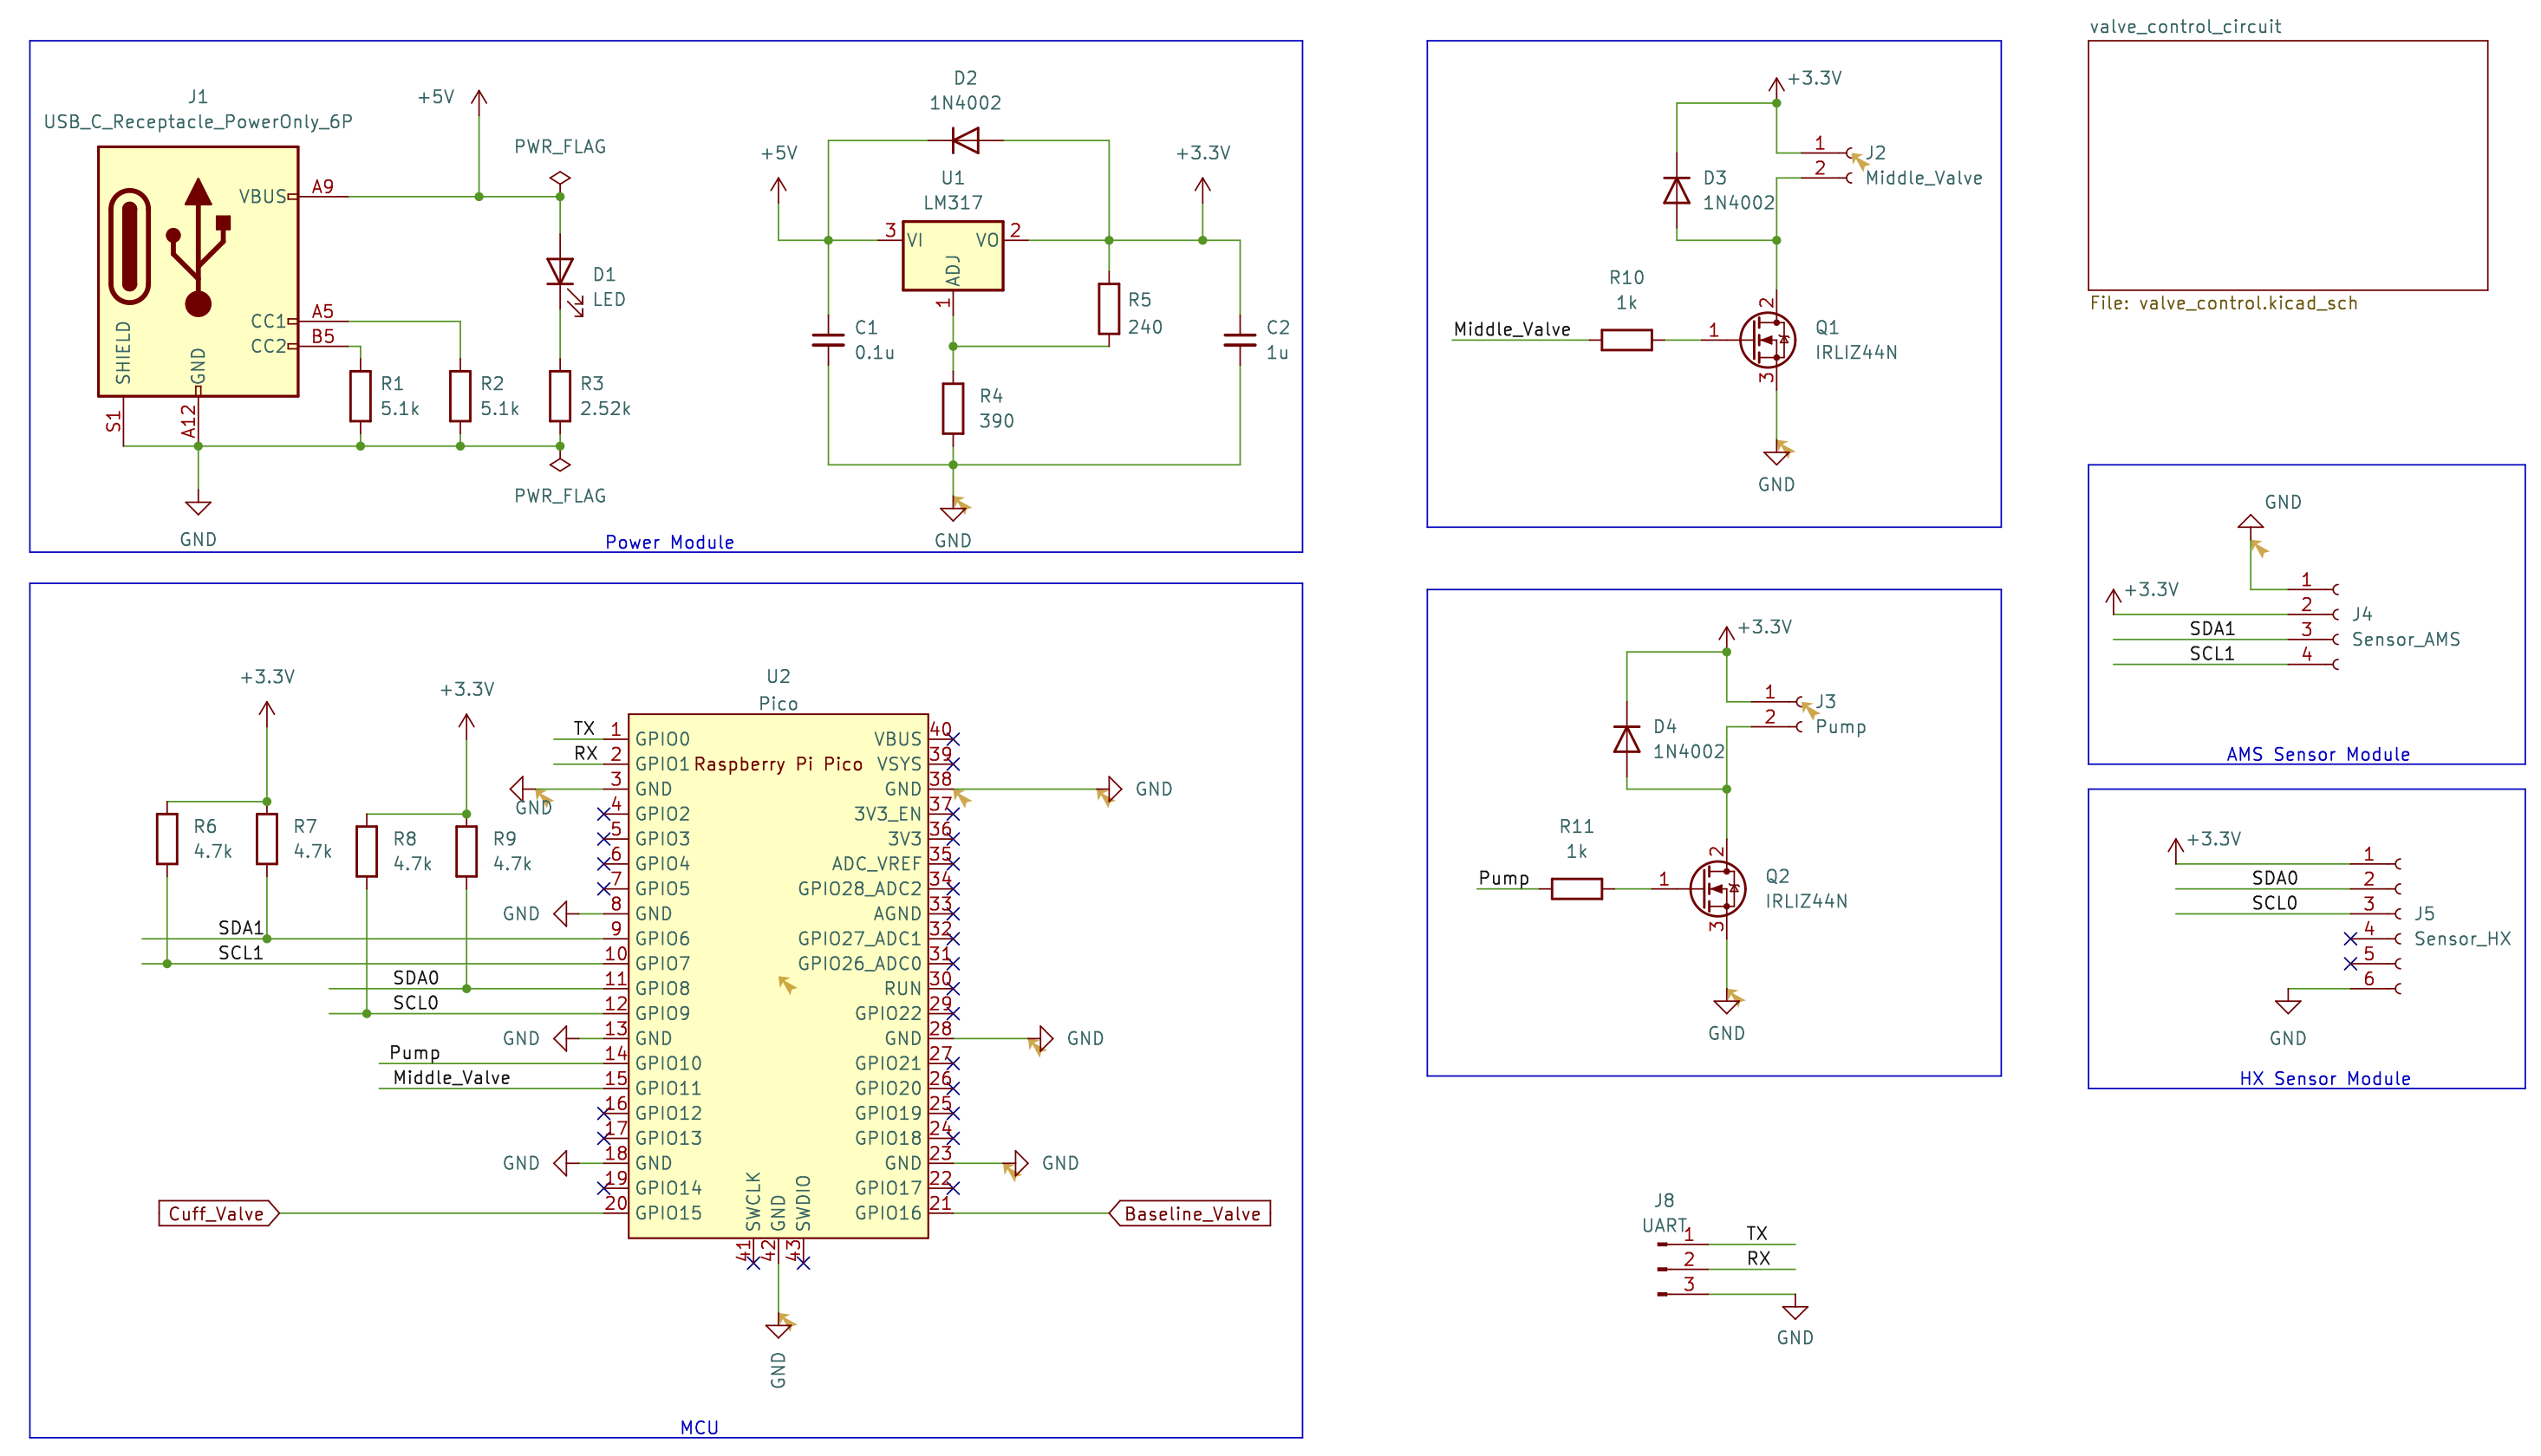
\includegraphics[width=0.75\textwidth]{img/schematic_diff-1.png}
    \caption{a nice plot}
    \label{fig:mesh1}
\end{figure}

\begin{figure}[h]
    \centering
    \captionsetup{justification=centering}
    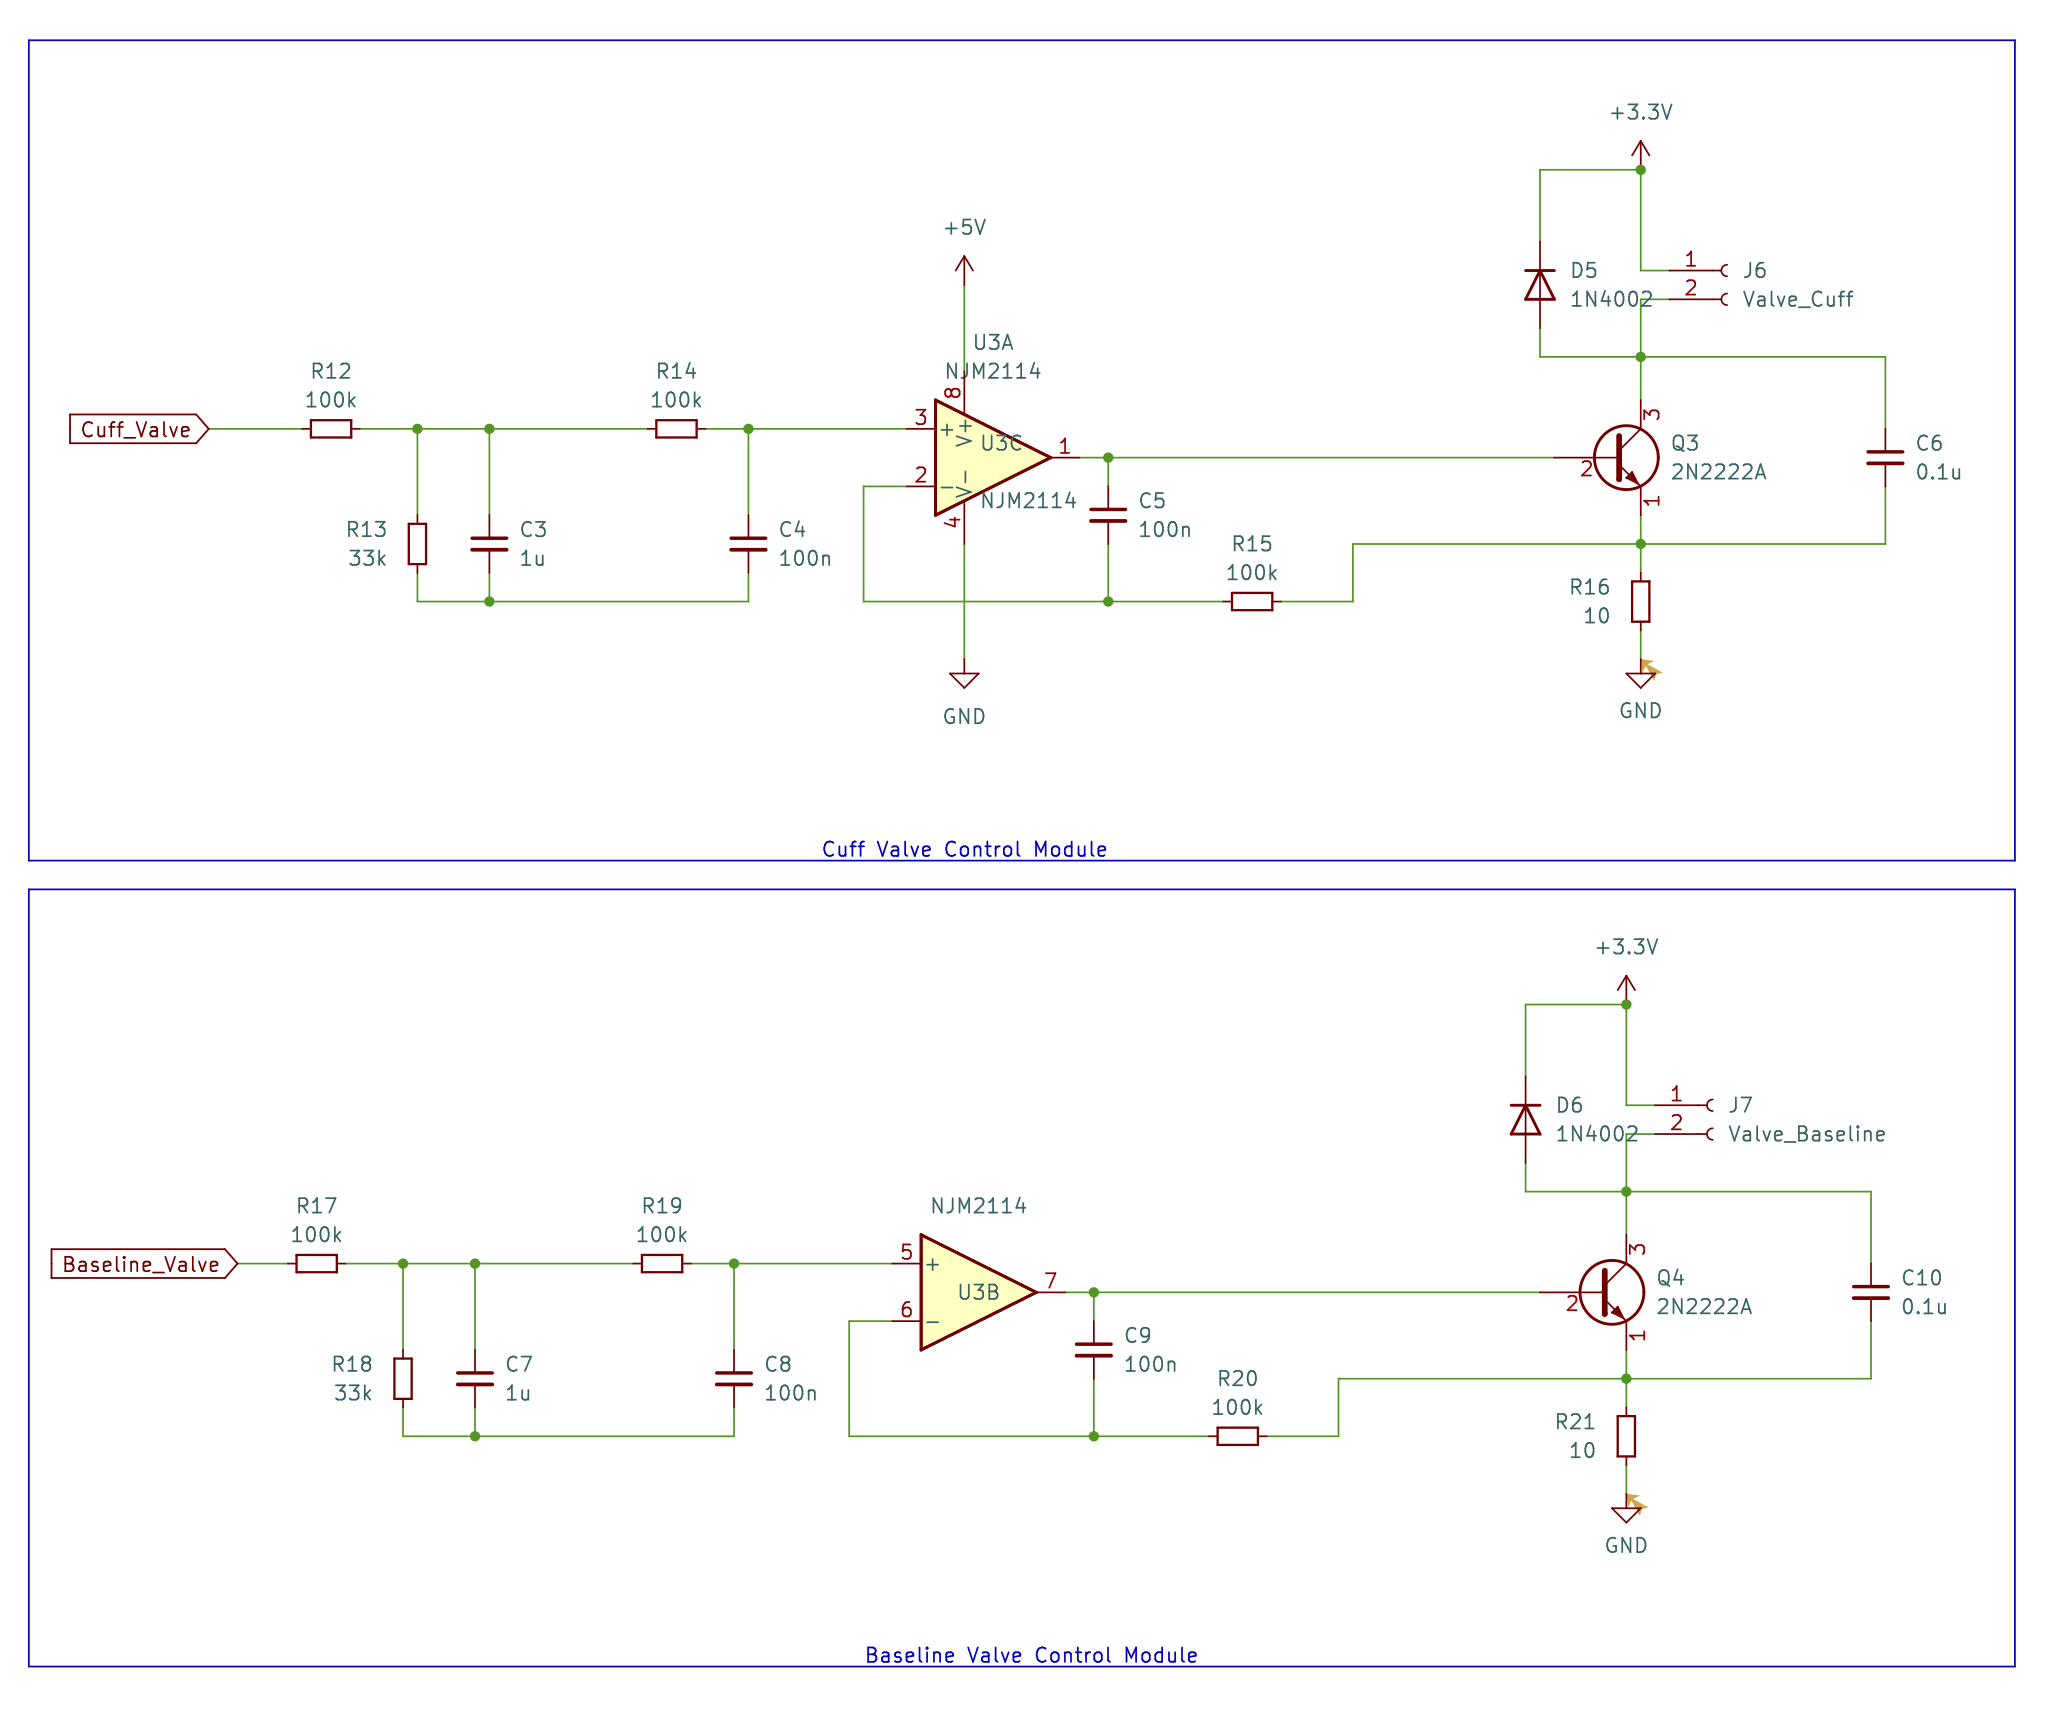
\includegraphics[width=0.75\textwidth]{img/schematic_diff-2.png}
    \caption{a nice plot}
    \label{fig:mesh1}
\end{figure}
